\section{Abstract Factory}

O padrão Abstract Factory define uma família 
de objetos relacionados e uma interface para 
criá-los, sem definir a implementação. Dessa 
forma, diferentes implementações desse 
conjunto de objetos podem ser utilizadas e 
as aplicações que utilizam esses objetos 
não precisam conhecer sua implementação.

O diagrama apresentado na figura \ref{abfactory_struct} 
demonstra a estrutura desse padrão, onde a 
interface AbstractFactory suporta as famílias 
ConcreteFactory1 e ConcreteFactory2, cada uma 
delas precisando implementar sua versão dos 
objetos AbstractProductA e AbstractProductB.

\begin{figure}[htb]
	\caption{\label{abfactory_struct}Estrutura do Abstract Factory}
	\begin{center}
	    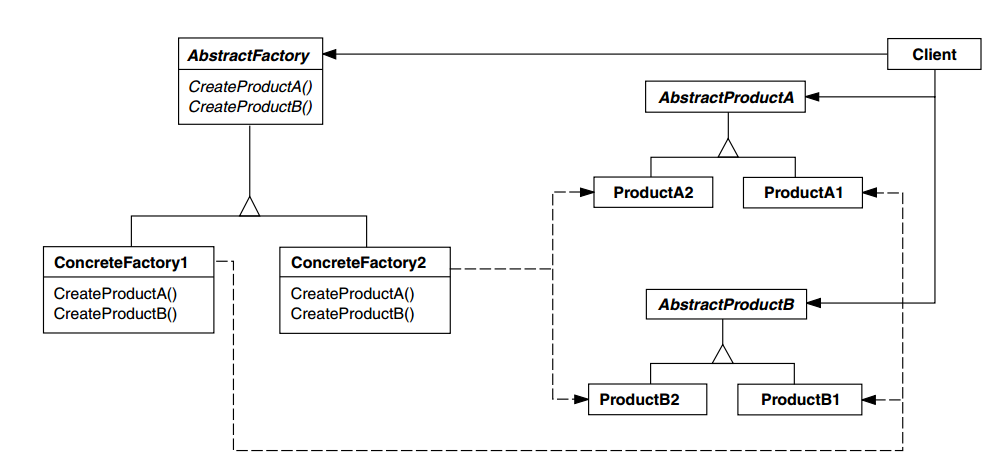
\includegraphics[scale=0.4]{5_padroes-contexto-funcional/5.1_criacionais/5.1.2_abstract-factory/diagram.png}
	\end{center}
\end{figure}

\subsection*{Exemplo Orientado a Objetos}

Como exemplo, é apresentado um \textit{toolkit} 
que suporta tipos diferentes de interação para 
seus \textit{widgets}, sendo 
os utilizados no exemplo Motif e Presentation 
Maneger (PM). Dessa forma, para que a aplicação 
não precise ser implementada pensando em todos 
os tipos diferentes de \textit{widgets}, é 
utilizado o padrão Abstract Factory para 
definir uma família de objetos de Widget 
diferente para cada tipo de interação. 

A implementação do padrão é demonstrada no 
diagrama de classes da figura \ref{abfactory_exemplo} 
e no código \ref{ooabfactory}. Uma interface 
WidgetFactory define as operações de criação 
de todos os \textit{widgets} possíveis, enquanto 
as classes MotifWidgetFactory e PMWidgetFactory 
implementam a criação dos mesmos de acordo 
com seus tipos de interação.

\begin{figure}[htb]
	\caption{\label{abfactory_exemplo}Exemplo de Abstract Factory}
	\begin{center}
	    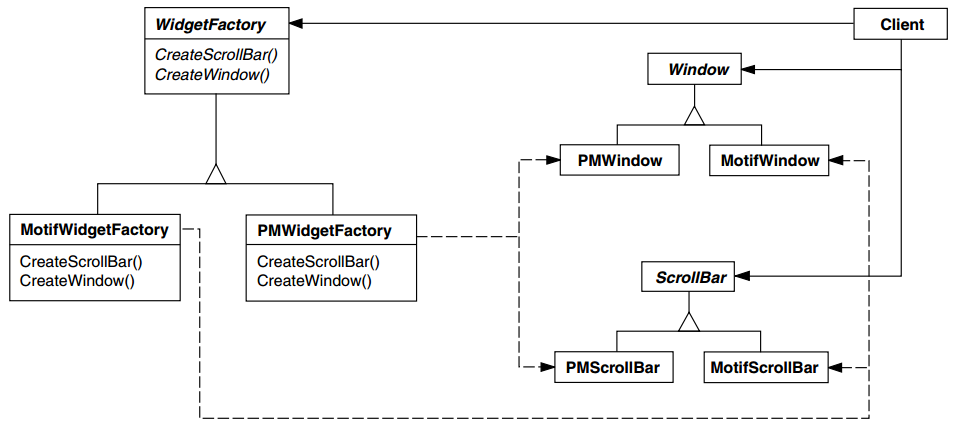
\includegraphics[scale=0.4]{5_padroes-contexto-funcional/5.1_criacionais/5.1.2_abstract-factory/exemplo_abfactory.png}
	\end{center}
\end{figure}

\begin{lstlisting}[caption={Abstract Factory Orientado a Objetos},label=ooabfactory]
	
	trait WidgetFactory {
		def createScrollBar() : ScrollBar
		def createWindow() : Window
	}

	trait Window 
	trait ScrollBar

	class MotifWidgetFactory() : WidgetFactory {
		def createScrollBar() : ScrollBar {
			return new MotifScrollBar()
		}

		def createWindow() : Window {
			return new MotifWindow()
		}
	}

	class PMWidgetFactory() : WidgetFactory {
		def createScrollBar() : ScrollBar {
			return new PMScrollBar()
		}

		def createWindow() : Window {
			return new PMWindow()
		}
	}

	class PMWindow() : Window {
		// Implementação de PMWindow
	}

	class MotifWindow() : Window {
		// Implementação de MotifWindow
	}

	class PMScrollBar() : ScrollBar {
		// Implementação de PMScrollBar
	}

	class MotifScrollBar() : ScrollBar {
		// Implementação de MotifScrollBar
	}

\end{lstlisting}



\subsection*{Contexto Funcional}

\begin{lstlisting}[caption={Abstract Factory Funcional},label=fpabfactory]
    
    

\end{lstlisting}